%lijst met inhoud in de marge
\input{../preamble}
\begin{document}

\section*{microsoft videocast}

\url{https://www.youtube.com/watch?v=F_Riqjdh2oM}

Begint met afspraken en herhaling linearire algebra:
Bit met waarde $0 \equiv \begin{pmatrix}
1\\
0
\end{pmatrix}
\equiv
\ket{0}$

Bit met waarde $1 \equiv 
\begin{pmatrix}
0\\
1
\end{pmatrix}
\equiv
\ket{1}$

(matrix)(kolomvector=(kolomvector)

(matrix)(matrix)=(matrix)

Beschouw de volgende vier klassieke operatoren op 1 bit:

Identiteit
$f(x)=x, 
I=\begin{pmatrix}
1&0\\
0&1
\end{pmatrix}
$

Negatie aka bitflip
$f(x)=not(x), X=\begin{pmatrix}
0&1\\
1&0
\end{pmatrix}
$

Set to 0
$f(x)=(0), S0=\begin{pmatrix}
1&1\\
0&0
\end{pmatrix}
$

Set to 1
$f(x)=(1), S1=\begin{pmatrix}
0&0\\
1&1
\end{pmatrix}
$

reversibele computing:
permutaties zijn reversibel overschrijven niet
I en X zijn reversible, S0 en S1 niet.
Quantum computers gebruiken alleen reversibele operatoren. Bovendien zijn alle quantumoperatoren reversibel. dt houdt in dat alle quantumoperatoren hun eigen  hun eigen inverse zijn.
$$XX=X^{-1}X=I$$
Makkelijk in te zien bij de bitflip: Een bitflip twee keer toepassen levertje het origineel.

tensorproduct:

$\begin{pmatrix}
x_0\\
x_1
\end{pmatrix}
\otimes
\begin{pmatrix}
y_0\\
y_1
\end{pmatrix}
=
\begin{pmatrix}
x_0 \begin{pmatrix}
y_0\\
y_1
\end{pmatrix}
\\
x_1\begin{pmatrix}
y_0\\
y_1
\end{pmatrix}

\end{pmatrix}
=
\begin{pmatrix}
x_0y_0\\
x_0y_1\\
x_1y_0\\
x_1y_1
\end{pmatrix}
$
 
Weergeven van meerdere klassieke bits
00
$\begin{pmatrix}
1\\
0
\end{pmatrix}
\otimes
\begin{pmatrix}
1\\
0
\end{pmatrix}
=
\begin{pmatrix}
1\\
0\\
0\\
0
\end{pmatrix}
$

$4_{10}=100_{2}=
\begin{pmatrix}
0\\
1
\end{pmatrix}
\otimes
\begin{pmatrix}
1\\
0
\end{pmatrix}
\otimes
\begin{pmatrix}
1\\
0
\end{pmatrix}
=
\begin{pmatrix}
0\\
0\\
0\\
0\\
1\\
0\\
0\\
0
\end{pmatrix}
$
Het product van $n$ bits is a vector of size $2^n$. 

CNOT gate werkt op twee bits. MSB is control bit LSB is het doelbit
Als control bit is 1 dan wordt doelbit geflipped. Als control bit is 0 dan onveranderd. Het controlbit is altijd onveranderd

$CNOT = 
\begin{pmatrix}
1&0&0&0\\
0&1&0&0\\
0&0&0&1\\
0&0&1&0\\
\end{pmatrix}
$

We schrijven het nog twee keer uit:

$
CNOT\ket{10}=CNOT
\begin{pmatrix}
\begin{pmatrix}
0\\
1
\end{pmatrix}
\otimes
\begin{pmatrix}
1\\
0
\end{pmatrix}
\end{pmatrix}
=
\begin{pmatrix}
1&0&0&0\\
0&1&0&0\\
0&0&0&1\\
0&0&1&0\\
\end{pmatrix}
\begin{pmatrix}
0\\
0\\
1\\
0
\end{pmatrix}
=
\begin{pmatrix}
0\\
0\\
0\\
1
\end{pmatrix}
=
\begin{pmatrix}
0\\
1
\end{pmatrix}
\otimes
\begin{pmatrix}
0\\
1
\end{pmatrix}
=
\ket{11}
$

$
CNOT\ket{11}=CNOT
\begin{pmatrix}
\begin{pmatrix}
0\\
1
\end{pmatrix}
\otimes
\begin{pmatrix}
0\\
1
\end{pmatrix}
\end{pmatrix}
=
\begin{pmatrix}
1&0&0&0\\
0&1&0&0\\
0&0&0&1\\
0&0&1&0\\
\end{pmatrix}
\begin{pmatrix}
0\\
0\\
0\\
1
\end{pmatrix}
=
\begin{pmatrix}
0\\
0\\
1\\
0
\end{pmatrix}
=
\begin{pmatrix}
0\\
1
\end{pmatrix}
\otimes
\begin{pmatrix}
1\\
0
\end{pmatrix}
=
\ket{10}
$

Ga zelf na dat $CNOT\ket{00} = \ket{00}$ en dat $CNOT\ket{01} = \ket{01}$

Een cbit is een speciale versie van een qubit. Een qubit is een representatie $\begin{pmatrix}
\alpha\\
\beta
\end{pmatrix}
$ waarbij $\alpha, \beta\in \mathbb{C}$

${|\alpha|}^2 +{|\beta|}^2 = 1$

De volgende 2-vectoren zijn voorbeelden van cbits:

$\begin{pmatrix}
\tfrac{1}{\sqrt{2}}\\
\tfrac{1}{\sqrt{2}}
\end{pmatrix}
$
, $\begin{pmatrix}
-\tfrac{1}{2}\\
\tfrac{\sqrt{3}}{2}
\end{pmatrix}
$
, $\begin{pmatrix}
1\\
0
\end{pmatrix}
$

de kansen stellen ($\tfrac{1}{2}, \tfrac{1}{2}$), (${\tfrac{1}{4}, \tfrac{3}{4}})$, en $(1,0)$ voor. 
Een qubit is in superpositie tot we een meting doen. Als we een qubit meten vervalt de toestand van de qubit tot $\ket{0}$ of $\ket{1}$

Een qubit $\begin{pmatrix}
\alpha\\
\beta
\end{pmatrix}
$
stort ineen $\ket{0}$ met kans $|\alpha|^2$ en tot $\ket{1}$ met kans $|\beta|^2$.

Bijvoorbeeld 
$\begin{pmatrix}
\tfrac{1}{2}\\
\tfrac{1}{2}
\end{pmatrix}
$
heeft gelijke kans op $\ket{0}$ en $\ket{1}$ (muntje opgooien)

$\begin{pmatrix}
1\\
0
\end{pmatrix}
$
levert met 100\% kans $\ket{0}$ op.

Al eerder gezien: meerdere qubits 
$\begin{pmatrix}
a\\
b
\end{pmatrix}
\otimes
\begin{pmatrix}
c\\
d
\end{pmatrix}
=
\begin{pmatrix}
ac\\
ad\\
bc\\
bd
\end{pmatrix}
$
met $|ac|^2+|ad|^2+|bc|^2+|bd|^2=1$
 
$\begin{pmatrix}
\tfrac{1}{\sqrt{2}}\\
\tfrac{1}{\sqrt{2}}
\end{pmatrix}
\otimes
\begin{pmatrix}
\tfrac{1}{\sqrt{2}}\\
\tfrac{1}{\sqrt{2}}
\end{pmatrix}
=
\begin{pmatrix}
\tfrac{1}{2}\\
\tfrac{1}{2}\\
\tfrac{1}{2}\\
\tfrac{1}{2}
\end{pmatrix}
$

Ga na dat het resultaat genormaliseerd is.
 Er is gelijke kans van $\tfrac{1}{4}$ op $\ket{00}$, $\ket{01}$,$\ket{10}$,$\ket{11}$.

Operaties werken ook op qubits net als op cbits bv X:

$f(x)=not(x)
\begin{pmatrix}
0&1\\
1&0
\end{pmatrix}
\begin{pmatrix}
-\tfrac{1}{2}\\
\tfrac{\sqrt{3}}{2}
\end{pmatrix}
=
\begin{pmatrix}
\tfrac{\sqrt{3}}{2}\\
-\tfrac{1}{2}
\end{pmatrix}
$

In quantum zijn er meer poorten mogelik.
Belangrijkste is de Hadamard gate:

$H\ket{1}=
\begin{pmatrix} 
\tfrac{1}{\sqrt{2}} & \tfrac{1}{\sqrt{2}}  \\ 
\tfrac{1}{\sqrt{2}} & -\tfrac{1}{\sqrt{2}} 
\end{pmatrix} 
\begin{pmatrix} 
0  \\ 
1
\end{pmatrix} 
=
\begin{pmatrix} 
\tfrac{1}{\sqrt{2}}\\
\tfrac{1}{\sqrt{2}}
\end{pmatrix} 
$

$H\ket{0}=
\begin{pmatrix} 
\tfrac{1}{\sqrt{2}} & \tfrac{1}{\sqrt{2}}  \\ 
\tfrac{1}{\sqrt{2}} & -\tfrac{1}{\sqrt{2}} 
\end{pmatrix} 
\begin{pmatrix} 
1  \\ 
0
\end{pmatrix} 
=
\begin{pmatrix} 
\tfrac{1}{\sqrt{2}}\\
-\tfrac{1}{\sqrt{2}}
\end{pmatrix} 
$
Als je de H-gate op het resultaat loslaat krijg je het origineel terug. Dat moet geen verassing zijn, want quantum gates zijn hun eigen inverse.

$H(H\ket{1})=
\begin{pmatrix} 
\tfrac{1}{\sqrt{2}} & \tfrac{1}{\sqrt{2}}  \\ 
\tfrac{1}{\sqrt{2}} & -\tfrac{1}{\sqrt{2}} 
\end{pmatrix} 
\begin{pmatrix} 
\tfrac{1}{\sqrt{2}}  \\ 
\tfrac{1}{\sqrt{2}}
\end{pmatrix} 
=
\begin{pmatrix} 
1\\
0
\end{pmatrix} 
$

$H(H\ket{0})=
\begin{pmatrix} 
\tfrac{1}{\sqrt{2}} & \tfrac{1}{\sqrt{2}}  \\ 
\tfrac{1}{\sqrt{2}} & -\tfrac{1}{\sqrt{2}} 
\end{pmatrix} 
\begin{pmatrix} 
\tfrac{1}{\sqrt{2}}  \\ 
\tfrac{1}{\sqrt{2}}
\end{pmatrix} 
=
\begin{pmatrix} 
0\\
1
\end{pmatrix} 
$

We kunnen uitgaan van een klasiek bit. Het in superpositie brengen, daarmee zijn we de quantumcomputer binnengekomen. We kunnen ook weer uit superpositie treden zonder te meten! Hieroor kan quantumcomputing deterministitsch worden ipv probabilistisch.

NB Een quantumcomputer kan alle klassieke operaties uitvoeren als je enen en nullen gebruikt voor de co\:efficienten.

De actie van gates kan je in een state machine weergeven zie fig. 
\marginpar{\vspace{0cm}\includegraphics[width=0.95\marginparwidth]{./img/statemachineXH.png}
 \captionof{figure}{Statemachine van X- en H- gate. (maak hier een tikzpicture)
 \label {fig:StateXH}}}
Merk op dat de de symmetrie. Met een keer spiegelen breng je de afbeelding weer terug tot het origineel. Met de hulp van deze deze statemachines hoef je niet meer al die matrixen uit te rekenen. Als je complexe getallen gebruikt wordt de voorstelling een bol (Bloch), maar blijft geldig.

\marginpar{\vspace{0cm}\includegraphics[width=0.95\marginparwidth]{./img/qcircuit.png}
 \captionof{figure}{quantum circuit.
 \label {fig:qcircuit}}}

recap:
\begin{itemize}[nosep]
\item  qubits zijn 2-vectoren met complexe coefficenten. Cbits zijn speciale gevallen van qubits (reeele coefficienten).
\item multi-bits systemen zijn tensor producten van enkele qubits. Idem voor cbits (n bits spannen een vectorruimte $2^n$ op 
\item Operaties op bits kun je met een matrix weergeven
\item de H-gate brengt $\ket{0}$
en $\ket{1}$ in gelijke superpositie, en terug.
\item elke gate is zijn eigen inverse.
\item Een gate twee keer (direct achter elkaar) uitgevoerd levert het origineel. 
\item Bits en operatoren kunnen op de eenheidscircel (blochbol) worden weergegeven als state machine.
\end{itemize}

NB. Een MZI kan je nu weergeven als een quantumcircuit. Spiegel is een bitflipper

$$H(X(H\ket{0}))=\ket{1}$$

\section*{Deutsch oracle}
Je krijgt een cadeau, een grote zwarte doos die een va de functies (S0, S1, I en X)  op \'e\'en bit kan uitvoeren. Je weet niet welke functie in de doos zit, maar je kan inputs proberen en de outputs observeren. Hoeveel ondervragingen moet je doen om er achter te komen welke functie er in de doos zit op een klasssieke computer? Hoeveel op een quantum computer?

klassiek: twee metingen nodig:
stuur een $\ket{0}$ in kijk wat er uit komt, Stuur een $\ket{1}$
in en kijk wat er uit komt. 
Op een qcomputer ook twee, want je hebt twee bits nodig om vier dingen te onderscheiden, maar 

\begin{itemize}[nosep]
\item Als je wilt weten of de functie constant (S0 en S1) is of variabel (I en X)
\item Hoeveel ondervragingen heb je nodig op een klasssieke computer en hoeveel op een quantum computer?
\end{itemize}
Klassiek zijn hiervoor nog steeds twee queries nodig, maar in quantum maar \'e\'en. We gebruiken de kracht van superpositie.

Hoe zien de functies er uit op een quantumcomputer. Gelijke een prbleem met S0 en S1 Deze zijn niet reversibel.

Hoe maak je niet-reversibele functies reversibel.
Oplossing: voeg een qubit toe waarop de functie wordt toegepast.
\marginpar{\vspace{0cm}\includegraphics[width=0.95\marginparwidth]{./img/deutsch.png}
 \captionof{figure}{een extra bit.
 \label {fig:deutsch}}}

[video t=36:08]

$\ket{x} \rightarrow f(\ket{x})$

\Qcircuit @C=1em @R=.7em {
& \gate{X} & \qw
}
\vspace{1cm}

\begin{center}
\Qcircuit @C=1em @R=2em {
\lstick{input} & \ustick{\ket{x}}& \qw & \gate{BB} & \qw & \qw & \ustick{\ket{f(x)}} & \rstick{output}
}
\end{center}
\vspace{1cm}
We bouwen de volgende testmachine. We bieden twee bits tegelijk aan. \textit{De namen input en output van de kanalen zijn verwarrend hier. Wat de machine volgens mij weergeeft is een BB met twee draadjes er aan. Links en rechts in de figuur geven de toestand voor en na de meting weer.} Op het MSB (input) staat onze testwaarde, op het LSB (output) bieden we $\ket{0}$ aan. We laten het input bit onveranderd, en lezen de functiewaarde van het output-bit.
\begin{center}
\Qcircuit @C=1em @R=2em {
\lstick{output} & \ustick{\ket{0}}& \qw & \multigate{1}{BB} & \qw & \qw & \ustick{\ket{f(x)}} & \rstick{output}\\
\lstick{input} & \ustick{\ket{x}} & \qw & \ghost{BB} & \qw & \qw & \ustick{\ket{x}}&  \rstick{input}
}
\end{center}
We testen vervolgens onze functies


\subsection*{Set-0}
Controleer dat 
$\ket{0} \rightarrow \ket{0}$ en 
$\ket{1} \rightarrow \ket{0}$

\vspace{0.5cm}
\Qcircuit @C=1em @R=2em {
\lstick{output} & \ustick{\ket{0}}& \qw & \qw & \qw & \qw & \ustick{\ket{0}} & \rstick{output}\\
\lstick{input} & \ustick{\ket{x}} & \qw & \qw & \qw & \qw & \ustick{\ket{x}}&  \rstick{input}
}

\subsection*{Set-1}
\vspace{0.5cm}
\Qcircuit @C=1em @R=2em {
\lstick{output} & \ustick{\ket{0}}& \qw & \gate{X} & \qw & \qw & \ustick{\ket{1}} & \rstick{output}\\
\lstick{input} & \ustick{\ket{x}} & \qw & \qw & \qw & \qw & \ustick{\ket{x}}&  \rstick{input}
}

\vspace{0.5cm}
\subsection*{Identity} We gebruiken een CNOT gate. De onderste lijn is de CONTROL lijn, de bovense (output) is de target. Als input is $\ket{0}$ dan is de bovenste onveranderd, $\ket{0}$. Als input $\ket{1}$ is dan flipt het bovenste bit $\ket{1}$. check!
\vspace{0.5cm}
\Qcircuit @C=1em @R=2em {
\lstick{output} & \ustick{\ket{0}}& \qw & \targ & \qw & \qw & \ustick{\ket{x}} & \rstick{output}\\
\lstick{input} & \ustick{\ket{x}} & \qw & \ctrl{-1} & \qw & \qw & \ustick{\ket{x}}&  \rstick{input}
}

\subsection{Bitflip} is makkelijk uit de identiteit te maken. Gewoon een X-gate toevoegen.
\vspace{0.5cm}
\Qcircuit @C=1em @R=2em {
\lstick{output} & \ustick{\ket{0}}& \qw & \targ & \gate{X} & \qw & \qw & \ustick{\ket{\lnot x}} & \rstick{output}\\
\lstick{input} & \ustick{\ket{x}} & \qw & \ctrl{-1} & \qw & \qw & \qw & \ustick{\ket{x}}&  \rstick{input}
}
\vspace{0.5cm}
Nu met de quantumcomputer: we bereiden het signaal voor voordat we het aan de input aanbieden. 
\begin{itemize}[nosep]
\item We bieden twee cbits aan op input en output. 
\item Beide kanalen gaan door een X-gate en enen H-gate waarmee ze in superpositie komen.
\item Met deze twee qubits testen we de BB.
\item De qubits gaan weer door een H-gate
\item Waarna een meting volgt.
 \end{itemize}
 
\vspace{0.5cm}
\begin{center}
\Qcircuit @C=1em @R=2em {
\lstick{output} & \ustick{\ket{0}}& \qw & \gate{X} & \gate{H} & 
\multigate{1}{BB}& \gate{H} & \meter & \qw & \ustick{\ket{f(x)}} & \rstick{output}\\
\lstick{input} & \ustick{\ket{x}} & \qw & \gate{X} & \gate{H} &
 \ghost{BB} & \gate{H} & \meter & \qw & \ustick{\ket{x}}&  \rstick{input}
}
\end{center}
Claim:
\begin{itemize}[nosep]
\item Als de BB functie constant is, dan is de output $\ket{11}$ na meting
\item Als de BB functie variabel is, dan is de output $\ket{01}$ na meting
\end{itemize}
NB input is het MSB

\marginpar{\vspace{0cm}\includegraphics[width=0.95\marginparwidth]{./img/deutschprepoc.png}
 \captionof{figure}{preprocessing.
 \label {fig:deutschpre}}}

\begin{center}  %DE manier om figuur te ontfloaten.
\leavevmode
\begin{tikzpicture}[scale=.5]
\def\vectsize{.7}
\def\radius{5cm}
\def\labelrad{4.cm}
\def\ketrad{5.5cm}
\def\arrowrad{3cm}
\draw (0,0) circle (\radius);
\foreach \x in {0,45,...,315} \filldraw (\x:\radius) circle (.1);

\node[scale=1] at (-5,5) {State machine}; 
\node[color=green] at (-5,4.5) {\footnotesize{X-gate}}; 
\node[color=red] at (-5,4) {\footnotesize{H-gate}}; 

\node[scale=1] at ( 90:\ketrad) {$\ket{1}$};
\node[scale=1] at (  0:\ketrad) {$\ket{0}$};
\node[scale=1] at (-90:\ketrad) {$\ket{1}$};
\node[scale=1] at (180:\ketrad) {$\ket{0}$};

%relaties X-gate
\draw[color=green, <->] (+90:\arrowrad) -- (0:\arrowrad);
\draw[color=green, <->] (+135:\arrowrad) -- (-45:\arrowrad);
\draw[color=green, <->] (+180:\arrowrad) -- (-90:\arrowrad);
\draw[color=green, <->] (4.3,4.3)+(240:.5) arc (240:570:.5);
\draw[color=green, <->] (-4.3,-4.3)+(60:.5) arc (60:390:.5);

%relaties Hadamard
\draw[color=red, <->] ( +45:\arrowrad) -- (0:\arrowrad);
\draw[color=red, <->] ( +90:\arrowrad) -- (-45:\arrowrad);
\draw[color=red, <->] (+135:\arrowrad) -- (-90:\arrowrad);
\draw[color=red, <->] (+180:\arrowrad) -- (225:\arrowrad);

%relatie cnot (kan eigelnlijk niet)
\draw[color=blue, <->] ( +45:\arrowrad) -- (-45:\arrowrad);

%startpunt
\draw[color=blue, ->] (5,-5) -- (4.2,-4.2);

\node[scale=\vectsize] at ( +90:\labelrad) {$\begin{pmatrix} 0 \\ 1 \end{pmatrix}$};
\node[scale=\vectsize] at ( +45:\labelrad) {$
\begin{pmatrix} \tfrac{1}{\sqrt{2}} \\ \tfrac{1}{\sqrt{2}} \end{pmatrix} $};
\node[scale=\vectsize] at (   0:\labelrad) {$\begin{pmatrix} 1 \\ 0 \end{pmatrix}$};
\node[scale=\vectsize] at ( -45:\labelrad) {$
\begin{pmatrix} \tfrac{1}{\sqrt{2}}  \\ \tfrac{-1}{\sqrt{2}} \end{pmatrix} $};
\node[scale=\vectsize] at ( -90:\labelrad) {$\begin{pmatrix} 0 \\ -1 \end{pmatrix}$};
\node[scale=\vectsize] at (-135:\labelrad) {$
\begin{pmatrix} \tfrac{-1}{\sqrt{2}}  \\ \tfrac{-1}{\sqrt{2}} \end{pmatrix} $};
\node[scale=\vectsize] at ( 180:\labelrad) {$\begin{pmatrix} -1\\ 0 \end{pmatrix}$};
\node[scale=\vectsize] at ( 135:\labelrad) {$
\begin{pmatrix} \tfrac{-1}{\sqrt{2}}  \\ \tfrac{1}{\sqrt{2}} \end{pmatrix} $};
\end{tikzpicture}
\captionof{figure}{State machine voor X-gate en H-gate $\alpha=0, \beta=1$. \label{fig:statedeutsch}}
\end{center}

Er is een spiegelsymmetrie voor elke poort. Net als bij een spiegeloperatie is een poort zijn eigen inverse. 
Alle 1-bit operaties kun je doen door over de eenheidcirkel te hoppen.

Probleem met de S0 en S1 gate: zij zijn niet  reversibel. Truuk: introduceer een extr bit. De nieuwe BB dlaat het input qubit onveranderd,, de functiewaarde wordt naar output geschreven.

Je kunt de BB met 4x4 matrices representeren, maar je kunt ook state machines gebruiken.

Test de vier funcites;
We bieden $\ket{00}$ aan.
Aan de ingang van de BB komt op beide kanalen $
\begin{pmatrix} \tfrac{1}{\sqrt{2}}  \\ \tfrac{-1}{\sqrt{2}} \end{pmatrix} $ te staan. (zie pijl in fig.). 
We lopen de vier functies af:

S0: laat de beide kanalen ongewijzigd. De H-gate na de BB beeldt de zowel de output als de input op 1 af.
Resultaat: (0,0) $\overset{S0}{\rightarrow}$ (1,1)

S1: Het output kanaal wordt geflipt, de H-gate beeldt op $
\begin{pmatrix} 0 \\ -1 \end{pmatrix}$ af. Voor een meting moeten we het kwadraat van de abs. waarde nemen: 1.
Met het inputkanaal gebeurt niets in de BB. Na de BB nog een H-gate toepassen: levert: $\ket{1}$
Resultaat: (0,0) $\overset{S0}{\rightarrow}$ (1,1)

I: Dit is wat meer werk. Hiervoor moeten we de CNOT operatie nader bekijken. CNOT werkt op twee bits. Voor cbits weten we al wat de CNOT operatie op levert, maar voor qubits nog niet. Laten we het gewoon uitschrijven voor onze input. 

De actie van CNOT is in het algemeen niet in de state machine weer te geven omdat de actie afhankelijk is van twee bits. Voor de onze situatie kunnen we het uitrekenen:

Het tensorproduct mag je niet omdraaien. Het is niet commutatief. De gebruikte vorm is $input \otimes output$

$
C\begin{pmatrix}
\begin{pmatrix} \tfrac{1}{\sqrt{2}}  \\ \tfrac{-1}{\sqrt{2}} \end{pmatrix}
\otimes
\begin{pmatrix} \tfrac{1}{\sqrt{2}}  \\ \tfrac{-1}{\sqrt{2}} \end{pmatrix}
\end{pmatrix}
=
C
\begin{pmatrix}
\tfrac{1}{2}\\
\tfrac{-1}{2}\\
\tfrac{-1}{2}\\
\tfrac{1}{2}
\end{pmatrix}
=
$

$
\tfrac{1}{2}
\begin{pmatrix}
1&0&0&0\\
0&1&0&0\\
0&0&0&1\\
0&0&1&0\\
\end{pmatrix}
\begin{pmatrix}
1\\
-1\\
-1\\
1
\end{pmatrix}
=
\tfrac{1}{2}
\begin{pmatrix}
1\\
-1\\
1\\
-1
\end{pmatrix}
=
\begin{pmatrix} \tfrac{1}{\sqrt{2}}  \\ \tfrac{1}{\sqrt{2}} \end{pmatrix}
\otimes
\begin{pmatrix} \tfrac{1}{\sqrt{2}}  \\ \tfrac{-1}{\sqrt{2}} \end{pmatrix}
$

De CNOT levert het resultaat $\ket{01}$.

\subsection*{bitflip}.
Net als bij de identiteit wordt eerst een CNOT toegepast.Voor de intput levert dat $\ket{0}$ op. De CNOT laat ook in dit geval onveranderd, maar wordt nog door een bitflip gehaald. Na de laatste H-gate wordt de output op $\ket{1}$ afgebeeld. Resultaat: $\ket{01}$



\subsection*{Verstrengeling}

Stel we hebben twee qubits in de volgende toestand
$
\begin{pmatrix}
a  \\ 
b
\end{pmatrix}
\otimes
\begin{pmatrix}
c  \\ 
d
\end{pmatrix}
=
\begin{pmatrix} \tfrac{1}{\sqrt{2}}  \\ 
0 \\
0\\
\tfrac{1}{\sqrt{2}} 
\end{pmatrix}
$

$ac=\tfrac{1}{\sqrt{2}}$
$ad=0$
$bc=0$
$bd=\tfrac{1}{\sqrt{2}}$

Dit stelsel is niet oplosbaar. Je kunt het niet ontbinden in twee bits. De toestanden zijn dan verstrengeld. De coefficenten leren je dat dit een even grote kans om ineen te storten tot $\ket{00}$ en $\ket{11}$.

Zo'n toestand is eenvoudig te maken.

\vspace{0.5cm}
\Qcircuit @C=1em @R=2em {
\ustick{\ket{0}}& \qw & \targ & \qw & \qw & \ustick{\ket{}}\\
\ustick{\ket{0}} & \gate{H} & \ctrl{-1} & \qw & \qw & \ustick{}
}
\vspace{0.5cm}

$
C\begin{pmatrix}
\begin{pmatrix} 1  \\ 0 \end{pmatrix}
\otimes
H\begin{pmatrix}
\begin{pmatrix} 1  \\ 0 \end{pmatrix}
\end{pmatrix}
\end{pmatrix}
=
C
\begin{pmatrix}
\begin{pmatrix}
\tfrac{1}{\sqrt{2}}\\
\tfrac{1}{\sqrt{2}}
\end{pmatrix}
\otimes
\begin{pmatrix}
1\\
0
\end{pmatrix}
\end{pmatrix}
=
$

$
\begin{pmatrix}
1&0&0&0\\
0&1&0&0\\
0&0&0&1\\
0&0&1&0\\
\end{pmatrix}
\begin{pmatrix}
\tfrac{1}{\sqrt{2}}\\
0\\
\tfrac{1}{\sqrt{2}}\\
0
\end{pmatrix}
=
\begin{pmatrix}
\tfrac{1}{\sqrt{2}}\\
0\\
0\\
\tfrac{1}{\sqrt{2}}
\end{pmatrix}
$

Nu gaat er een wereld open. Twee qubits zijn verstrengeld. Maakt niet uit op welke afstand. Als een van hen gemten wordt valt de toestand van de ander instantaan op zijn plek (experiment atoomklokken 2013?). 

Spooky action at a distance.
EPR

Teleportatie
[dit is niet goed uitgewerkt in de presentatie]

\vspace{1cm}
\Qcircuit @C=1em @R=2em {
\lstick{T} & \ustick{\ket{\Psi}} & \qw     & \qw       & \targ     & \gate{H}   & \qw      & \meter \cwx[2] \\
\lstick{A} & \ustick{\ket{0}}    & \gate{H}& \targ     & \ctrl{-1} & \qw        & \meter \cwx[1]  \\
\lstick{B} & \ustick{\ket{0}}    & \qw     & \ctrl{-1} & \qw       & \qw        & \gate{X} & \gate{Z} & \qw & \ustick{\ket{\Psi}}
}


\end{document}